\documentclass[aspectratio=169,10pt]{beamer}

\usepackage[utf8]{inputenc}
\usepackage{amsmath,amssymb,amsfonts}
\usepackage{graphicx}
\usepackage{booktabs}
\usepackage{tabularx}
\usepackage{array}
\usepackage{xcolor}

% Enforce uniform margins on all 4 sides
\setbeamersize{text margin left=0.8cm, text margin right=0.8cm}
\setbeamertemplate{navigation symbols}{}
\setbeamertemplate{headline}{}

% Color Palette inspired by modern statistical monitoring slides
\definecolor{navybg}{RGB}{14, 26, 48}        % Deep Midnight Navy (Title, Section, Summary slides)
\definecolor{headernavy}{RGB}{15, 28, 54}     % Slide Title Dark Navy
\definecolor{subgray}{RGB}{100, 116, 139}     % Subtitle Slate Gray
\definecolor{accentcyan}{RGB}{45, 175, 195}   % Teal / Cyan accent
\definecolor{accentblue}{RGB}{24, 76, 160}    % Primary Blue accent
\definecolor{accentred}{RGB}{195, 35, 45}     % Crimson Red accent
\definecolor{accentgreen}{RGB}{20, 135, 75}   % Emerald Green accent
\definecolor{cardbg}{RGB}{246, 248, 252}      % Soft Card Background
\definecolor{cardborder}{RGB}{226, 232, 240}  % Card Border
\definecolor{textdark}{RGB}{30, 41, 59}       % Dark Slate Body Text

\setbeamercolor{normal text}{fg=textdark}

% Minimalist footline with slide number at bottom right
\setbeamertemplate{footline}{
  \ifnum\thepage>1
    \vspace{-0.45cm}
    \hfill {\scriptsize \color{subgray} \insertframenumber{} / \inserttotalframenumber} \hspace{0.8cm}
    \vspace{0.25cm}
  \fi
}

\begin{document}

% =========================================================
% Slide 1: Title Slide (Deep Navy)
% =========================================================
{
\setbeamercolor{background canvas}{bg=navybg}
\begin{frame}[c,plain]
  \centering
  {\Large \textbf{\color{white} Bayesian Data Analysis of the German Tank Problem}}\\[0.22cm]
  {\large \textbf{\color{white} Theoretical Properties, Simulation Benchmarks, and Real-World Stress-Testing}}\\[0.18cm]
  {\small \color{accentcyan} Inferring Discrete Ceilings, Decision Theory, and Operational Assumption Violations}\\[0.65cm]
  
  {\normalsize \textbf{\color{white} Aklanta Borah \quad Amartya Amritanshu \quad Rajveer Vora}}\\[0.12cm]
  {\footnotesize \color{white!80} Indian Statistical Institute, Kolkata}\\[0.08cm]
  {\scriptsize \color{white!50} Nov 2026}
\end{frame}
}

% =========================================================
% Slide 2: Historical Context: Statistical Intelligence in WWII
% =========================================================
\begin{frame}[c]
  \begin{center}
    {\large \textbf{\color{headernavy} Historical Context: Statistical Intelligence in WWII}}\\[0.10cm]
    {\scriptsize \color{subgray} Objective: Infer the unknown total number of tanks produced, $N$, using a small sample of observed serial numbers.}
  \end{center}
  \vspace{0.35cm}
  
  \begin{columns}[t,onlytextwidth]
    \begin{column}{0.31\textwidth}
      {\small \textbf{\color{headernavy} 1. Espionage Inflation}}\\[0.08cm]
      {\scriptsize Conventional military intelligence relied on spy networks and captured prisoners, drastically overestimating production by \textbf{4.5--8.2$\times$} (1,000--1,550 tanks/mo).}
    \end{column}
    
    \begin{column}{0.31\textwidth}
      {\small \textbf{\color{headernavy} 2. Order Statistics}}\\[0.08cm]
      {\scriptsize Allied statisticians analyzed captured chassis and gearbox serials ($k \approx 5$--$50$), mathematically estimating production at \textbf{169--327} tanks/mo.}
    \end{column}
    
    \begin{column}{0.31\textwidth}
      {\small \textbf{\color{headernavy} 3. Speer Ministry Ledgers}}\\[0.08cm]
      {\scriptsize Post-war Albert Speer production records confirmed statistical estimates converged within \textbf{4\%--10\%} of actual production.}
    \end{column}
  \end{columns}
  
  \vspace{0.25cm}
  \begin{center}
    \resizebox{0.82\textwidth}{!}{
    \begin{tabular}{lcccc}
      \toprule
      \textbf{Production Month} & \textbf{Conventional Spy Est.} & \textbf{Statistical Est. ($\hat{N}$)} & \textbf{Speer Ministry True ($N$)} & \textbf{Statistical Error} \\
      \midrule
      June 1940 (Early Marks)   & 1,000 & \textbf{169} & 122 & $+38.5\%$ \\
      June 1941 (Panzer III/IV) & 1,550 & \textbf{244} & 271 & $\mathbf{-9.9\%}$ \\
      August 1942 (Panzer III/IV) & 1,550 & \textbf{327} & 342 & $\mathbf{-4.4\%}$ \\
      \bottomrule
    \end{tabular}}
  \end{center}
  
  \vspace{0.18cm}
  \begin{center}
    {\footnotesize \textbf{\color{headernavy} Core Inferential Objective: } \textit{Infer the unknown population ceiling $N$, moving beyond point estimates to complete uncertainty quantification.}}
  \end{center}
\end{frame}

% =========================================================
% Slide 3: Mathematical Formulation: The Observation Model
% =========================================================
\begin{frame}[c]
  \begin{center}
    {\large \textbf{\color{headernavy} Mathematical Formulation: Data, Parameter, and Likelihood}}\\[0.10cm]
    {\scriptsize \color{subgray} Explicitly separating what is observed from the unknown parameter we seek to infer.}
  \end{center}
  \vspace{0.38cm}
  
  \begin{columns}[t,onlytextwidth]
    \begin{column}{0.48\textwidth}
      {\small \textbf{\color{accentblue} The Data-Generating Mechanism}}\\[0.08cm]
      {\scriptsize Serials drawn by simple random sampling without replacement:
      \begin{equation*}
        S_1, \ldots, S_k \overset{\mathrm{SRSWOR}}{\sim} \{1, 2, \ldots, N\}
      \end{equation*}
      \begin{itemize}
        \setlength{\itemsep}{0.08cm}
        \item \textbf{Observed Data:} $D = \{s_1, \ldots, s_k\}$ with sample size $k$.
        \item \textbf{Order Statistics:} $1 \le s_{(1)} < s_{(2)} < \dots < s_{(k)} = m$.
        \item \textbf{Sample Maximum:} $m = \max(s_1, \ldots, s_k)$.
        \item \textbf{Physical Boundary:} $N \ge m$ is an absolute physical constraint.
      \end{itemize}}
    \end{column}
    
    \begin{column}{0.48\textwidth}
      {\small \textbf{\color{headernavy} Inferential Target \& Unordered Likelihood}}\\[0.08cm]
      {\scriptsize
      \begin{itemize}
        \setlength{\itemsep}{0.08cm}
        \item \textbf{Inferential Target:} The target is the unknown population ceiling $N \in \mathbb{N}_{\ge m}$, \textit{not the individual serial numbers}.
        \item The serial numbers $D$ are observed data; $N$ is the unknown quantity we want to learn about.
      \end{itemize}
      \begin{equation*}
        P(D \mid N, k) = \frac{1}{\binom{N}{k}} \mathbb{I}(N \ge m)
      \end{equation*}
      \begin{itemize}
        \setlength{\itemsep}{0.08cm}
        \item Likelihood is strictly zero for all $N < m$.
        \item Sample maximum $m$ captures all sample dependence on $N$.
      \end{itemize}}
    \end{column}
  \end{columns}
  
  \vspace{0.25cm}
  \begin{center}
    {\footnotesize \textbf{\color{headernavy} Key Insight: } \textit{The serial numbers are observed evidence; the population ceiling $N$ is the unknown inferential target.}}
  \end{center}
\end{frame}

% =========================================================
% Slide 4: Classical Solution: The UMVUE & Its Limitations
% =========================================================
\begin{frame}[c]
  \begin{center}
    {\large \textbf{\color{headernavy} Classical Solution: The UMVUE \& Its Limitations}}\\[0.10cm]
    {\scriptsize \color{subgray} Frequentist point estimation achieves repeated-sampling unbiasedness but provides no posterior distribution.}
  \end{center}
  \vspace{0.38cm}
  
  \begin{columns}[t,onlytextwidth]
    \begin{column}{0.48\textwidth}
      {\small \textbf{\color{accentgreen} The UMVUE Estimator}}\\[0.08cm]
      {\scriptsize By the likelihood ratio criterion for minimal sufficiency (Bahadur, 1954), $M = \max_i S_i$ is complete and minimal sufficient.
      \begin{equation*}
        \widehat{N}_{\mathrm{UMVUE}} = m \left(1 + \frac{1}{k}\right) - 1
      \end{equation*}
      \begin{equation*}
        \operatorname{Var}(\widehat{N}_{\mathrm{UMVUE}}) = \frac{(N-k)(N+1)}{k(k+2)}
      \end{equation*}
      \begin{itemize}
        \setlength{\itemsep}{0.06cm}
        \item Unbiased across hypothetical repeated samples ($\mathbb{E}[\widehat{N}] = N$).
        \item Simple closed-form computation requiring only $m$ and $k$.
      \end{itemize}}
    \end{column}
    
    \begin{column}{0.48\textwidth}
      {\small \textbf{\color{accentred} Fundamental Limitations of Classical Approach}}\\[0.08cm]
      {\scriptsize
      \begin{itemize}
        \setlength{\itemsep}{0.10cm}
        \item \textbf{No Posterior Uncertainty Distribution:} The classical approach constructs a point estimator that is unbiased over repeated samples. It does not provide a posterior distribution describing uncertainty about $N$ given this specific sample.
        \item \textbf{Boundary Violations:} Asymptotic Wald intervals ($\widehat{N} \pm 1.96 \cdot \mathrm{SE}$) extend below $m$, placing mass on physically impossible values ($N < m$).
        \item \textbf{Inflexible to Decision Costs:} Cannot adapt to asymmetric operational losses where underestimation carries disastrous strategic costs.
      \end{itemize}}
    \end{column}
  \end{columns}
  
  \vspace{0.25cm}
  \begin{center}
    {\footnotesize \textbf{\color{headernavy} Transition to Bayes: } \textit{Point estimators provide only an average; Bayesian inference constructs the full posterior distribution $P(N \mid D)$.}}
  \end{center}
\end{frame}

% =========================================================
% Slide 5: Section 01 Divider (Deep Navy)
% =========================================================
{
\setbeamercolor{background canvas}{bg=navybg}
\begin{frame}[c,plain]
  \centering
  {\scriptsize \textbf{\color{accentcyan} SECTION 01}}\\[0.25cm]
  {\LARGE \textbf{\color{white} Theoretical Properties \& Bayesian Foundations}}\\[0.35cm]
  {\small \color{white!70} Inferring the posterior distribution, reference priors, loss geometry, and boundary admissibility}
\end{frame}
}

% =========================================================
% Slide 6: Bayesian Inference: What Are We Trying to Infer?
% =========================================================
\begin{frame}[c]
  \begin{center}
    {\large \textbf{\color{headernavy} Bayesian Inference: What Are We Trying to Infer?}}\\[0.10cm]
    {\scriptsize \color{subgray} Establishing the inferential objective: moving from raw identifiers to an epistemic probability distribution.}
  \end{center}
  \vspace{0.35cm}
  
  \begin{columns}[t,onlytextwidth]
    \begin{column}{0.48\textwidth}
      {\small \textbf{\color{headernavy} 1. What Do We Know?}}\\[0.04cm]
      {\scriptsize
      \begin{itemize}
        \setlength{\itemsep}{0.04cm}
        \item The observed sample of serial numbers $D = \{s_1, \ldots, s_k\}$.
        \item The sample maximum $m = \max(s_1, \ldots, s_k)$.
        \item Physical fact: the population must satisfy $N \ge m$.
      \end{itemize}}
      \vspace{0.14cm}
      
      {\small \textbf{\color{accentred} 2. What Is Unknown?}}\\[0.04cm]
      {\scriptsize
      \begin{itemize}
        \setlength{\itemsep}{0.04cm}
        \item The true population ceiling $N \in \{m, m+1, m+2, \ldots\}$.
        \item We do not know how far above $m$ the true ceiling lies.
      \end{itemize}}
    \end{column}
    
    \begin{column}{0.48\textwidth}
      {\small \textbf{\color{accentblue} 3. What Does Bayesian Inference Give Us?}}\\[0.04cm]
      {\scriptsize A posterior distribution describing the probability of every possible population size, conditional on the observed data:
      \begin{equation*}
        \boxed{P(N = n \mid D)}
      \end{equation*}}
      \vspace{0.06cm}
      
      {\small \textbf{\color{accentgreen} 4. What Do We Do With This Distribution?}}\\[0.04cm]
      {\scriptsize
      \begin{itemize}
        \setlength{\itemsep}{0.04cm}
        \item Quantify uncertainty via exact credible intervals.
        \item Derive optimal point estimates tailored to specific loss functions.
        \item Make principled decisions accounting for risk asymmetry.
      \end{itemize}}
    \end{column}
  \end{columns}
  
  \vspace{0.25cm}
  \begin{center}
    \setlength{\fboxrule}{1pt}
    \fcolorbox{cardborder}{cardbg}{
      \parbox{0.94\textwidth}{\centering
        \scriptsize \textbf{\color{headernavy} Inferential Pipeline: }
        $\text{Observed Data } D = \{s_1, \dots, s_k\} \;\longrightarrow\; \mathbf{Posterior\;Distribution\;} P(N=n \mid D) \;\longrightarrow\; \text{Estimation \& Decision Rules } \widehat{N}_L$
      }
    }
  \end{center}
  
  \vspace{0.12cm}
  \begin{center}
    {\footnotesize \textbf{\color{headernavy} Core Message: } \textit{The posterior distribution itself is the primary inferential output; point estimates are derived afterwards.}}
  \end{center}
\end{frame}

% =========================================================
% Slide 7: Ingredients of Bayesian Inference: Likelihood, Prior, Posterior
% =========================================================
\begin{frame}[c]
  \begin{center}
    {\large \textbf{\color{headernavy} Ingredients of Bayesian Inference: Likelihood, Prior, Posterior}}\\[0.10cm]
    {\scriptsize \color{subgray} How observed evidence combines with prior assumptions to quantify uncertainty about $N$.}
  \end{center}
  \vspace{0.35cm}
  
  \begin{columns}[t,onlytextwidth]
    \begin{column}{0.31\textwidth}
      {\small \textbf{\color{accentblue} 1. Likelihood: Data Evidence}}\\[0.06cm]
      {\scriptsize What does the sample tell us about $N$?
      \begin{equation*}
        P(D \mid N = n) = \frac{1}{\binom{n}{k}} \mathbb{I}(n \ge m)
      \end{equation*}
      \begin{itemize}
        \setlength{\itemsep}{0.06cm}
        \item Measures the probability of observing $D$ under each candidate $n$.
        \item Equals \textbf{zero for $n < m$}: automatically assigns zero posterior probability to physically impossible population sizes.
      \end{itemize}}
    \end{column}
    
    \begin{column}{0.33\textwidth}
      {\small \textbf{\color{accentgreen} 2. Prior: Initial Assumptions}}\\[0.06cm]
      {\scriptsize What do we assume about $N$ before observing data?
      \begin{itemize}
        \setlength{\itemsep}{0.06cm}
        \item \textbf{Flat Prior ($\pi \propto 1$):} Assumes equal prior weight across all candidate integers.
        \item \textbf{Reciprocal Prior ($\pi \propto 1/n$):} Discrete analog of scale invariance; assigns equal mass to multiplicative decades/octaves ($\sum_A^{cA} \frac{1}{n} \approx \log c$).
      \end{itemize}}
    \end{column}
    
    \begin{column}{0.33\textwidth}
      {\small \textbf{\color{headernavy} 3. Posterior: Updated Belief}}\\[0.06cm]
      {\scriptsize What do we believe about $N$ after observing data?
      \begin{equation*}
        \boxed{P(N = n \mid D) = \frac{\binom{n}{k}^{-1} \pi(n)}{\sum_{j=m}^\infty \binom{j}{k}^{-1} \pi(j)}}
      \end{equation*}
      \begin{itemize}
        \setlength{\itemsep}{0.06cm}
        \item Combines serial evidence with prior structure.
        \item Quantifies epistemic uncertainty across all physically admissible $n \ge m$.
      \end{itemize}}
    \end{column}
  \end{columns}
  
  \vspace{0.30cm}
  \begin{center}
    {\footnotesize \textbf{\color{headernavy} Posterior Interpretation: } \textit{The posterior combines sample data with prior assumptions to assign exact probabilities to all candidate population sizes.}}
  \end{center}
\end{frame}

% =========================================================
% Slide 8: Discrete Posteriors: Derivation, Propriety & Moments
% =========================================================
\begin{frame}[c]
  \begin{center}
    {\large \textbf{\color{headernavy} Discrete Posteriors: Propriety \& Moment Existence Thresholds}}\\[0.10cm]
    {\scriptsize \color{subgray} Different prior assumptions produce different posterior distributions, even when the observed data remain unchanged.}
  \end{center}
  \vspace{0.32cm}
  
  \begin{columns}[t,onlytextwidth]
    \begin{column}{0.48\textwidth}
      {\small \textbf{\color{headernavy} Exact Discrete Posterior PMFs ($n \ge m$)}}\\[0.08cm]
      {\scriptsize
      \begin{itemize}
        \setlength{\itemsep}{0.08cm}
        \item \textbf{Flat Prior ($\pi \propto 1$):}
        \begin{equation*}
          P(N = n \mid m, k) = \frac{k - 1}{k} \frac{\binom{m-1}{k-1}}{\binom{n}{k}}
        \end{equation*}
        Normalizing constant telescopes exactly via negative hypergeometric summation.
        \item \textbf{Reciprocal Prior ($\pi \propto 1/n$):}
        \begin{equation*}
          P(N = n \mid m, k) = \frac{1}{Z(m,k)} \frac{1}{n \binom{n}{k}}
        \end{equation*}
        $Z(m,k) = \sum_{j=m}^\infty \frac{1}{j \binom{j}{k}}$ converges for all $k \ge 1$ (no simple closed form; evaluated numerically).
      \end{itemize}}
    \end{column}
    
    \begin{column}{0.48\textwidth}
      {\small \textbf{\color{accentblue} Moment Existence Thresholds \& Pareto Limit}}\\[0.08cm]
      {\scriptsize
      \begin{center}
        \resizebox{\linewidth}{!}{
        \begin{tabular}{lccc}
          \toprule
          \textbf{Prior Distribution} & \textbf{Proper Posterior} & \textbf{Finite Mean $\mathbb{E}[N]$} & \textbf{Finite Var $\operatorname{Var}(N)$} \\
          \midrule
          Flat Prior ($\pi \propto 1$)      & $k \ge 2$ & $k \ge 3$ ($\mathbb{E} = 2m-2$) & $k \ge 4$ \\
          Reciprocal Prior ($\pi \propto 1/n$) & \textbf{$k \ge 1$} & \textbf{$k \ge 2$} ($\mathbb{E} \approx 2m$) & \textbf{$k \ge 3$} \\
          \bottomrule
        \end{tabular}}
      \end{center}
      \vspace{0.08cm}
      \textbf{Continuous Pareto Limit ($N \gg k$):}
      \begin{equation*}
        p(N \mid m, k) \approx \frac{(k-1) m^{k-1}}{N^k}, \quad N \ge m
      \end{equation*}
      \begin{itemize}
        \setlength{\itemsep}{0.04cm}
        \item Cumulative CDF: $F(N) = 1 - (m/N)^{k-1}$.
        \item Median: $\widehat{N}_{\mathrm{med}} \approx m \cdot 2^{1/(k-1)}$.
      \end{itemize}}
    \end{column}
  \end{columns}
  
  \vspace{0.20cm}
  \begin{center}
    {\footnotesize \textbf{\color{headernavy} Theoretical Takeaway: } \textit{Reciprocal prior guarantees posterior propriety for all $k \ge 1$, whereas flat prior requires $k \ge 2$ for propriety and $k \ge 3$ for finite mean.}}
  \end{center}
\end{frame}

% =========================================================
% Slide 9: Estimating N from a Loss Function: Decision Theory
% =========================================================
\begin{frame}[c]
  \begin{center}
    {\large \textbf{\color{headernavy} Estimating $N$ from a Loss Function: Bayesian Decision Theory}}\\[0.10cm]
    {\scriptsize \color{subgray} A posterior distribution describes uncertainty, but a decision requires us to select a single estimate.}
  \end{center}
  \vspace{0.38cm}
  
  \begin{columns}[t,onlytextwidth]
    \begin{column}{0.48\textwidth}
      {\small \textbf{\color{headernavy} The Decision-Theoretic Framework}}\\[0.08cm]
      {\scriptsize
      \begin{itemize}
        \setlength{\itemsep}{0.08cm}
        \item The optimal estimate depends on the cost assigned to different estimation errors.
        \item Let $a \in \mathbb{N}_{\ge m}$ denote an estimation action.
        \item Loss function $L(N, a)$ quantifies the consequence of predicting $a$ when true population is $N$.
        \item \textbf{Posterior Expected Loss (Risk):}
        \begin{equation*}
          R(a) = \mathbb{E}[L(N, a) \mid D] = \sum_{n=m}^\infty L(n, a) P(N = n \mid D)
        \end{equation*}
        \item \textbf{Optimal Bayes Estimator:}
        \begin{equation*}
          \widehat{N}_L = \arg\min_a R(a)
        \end{equation*}
      \end{itemize}}
    \end{column}
    
    \begin{column}{0.48\textwidth}
      {\small \textbf{\color{accentblue} Example: Squared-Error Loss ($L_2$)}}\\[0.08cm]
      {\scriptsize When estimation errors are penalized quadratically:
      \begin{equation*}
        L(N, a) = (N - a)^2
      \end{equation*}
      \begin{equation*}
        R(a) = \mathbb{E}[(N - a)^2 \mid D] = \operatorname{Var}(N \mid D) + (\mathbb{E}[N \mid D] - a)^2
      \end{equation*}
      Setting the derivative to zero yields:
      \begin{equation*}
        \boxed{\widehat{N}_{L_2} = \mathbb{E}[N \mid D] \quad \text{(Posterior Mean)}}
      \end{equation*}
      \begin{itemize}
        \setlength{\itemsep}{0.06cm}
        \item The posterior mean is not "the" Bayesian estimate; it is optimal specifically for squared-error loss.
        \item If errors carry asymmetric costs, a different estimator is required.
      \end{itemize}}
    \end{column}
  \end{columns}
  
  \vspace{0.25cm}
  \begin{center}
    {\footnotesize \textbf{\color{headernavy} Core Rule: } \textit{Decisions follow inference: point estimators cannot be chosen without defining a loss function.}}
  \end{center}
\end{frame}

% =========================================================
% Slide 10: Loss Functions & Bayesian Estimators
% =========================================================
\begin{frame}[c]
  \begin{center}
    {\large \textbf{\color{headernavy} Loss Functions \& Bayesian Estimators: Matching Risk to Mission}}\\[0.10cm]
    {\scriptsize \color{subgray} Point estimators shift systematically with the decision-maker's loss geometry.}
  \end{center}
  \vspace{0.32cm}
  
  \begin{columns}[t,onlytextwidth]
    \begin{column}{0.24\textwidth}
      {\small \textbf{\color{accentred} 1. 0--1 Loss}}\\[0.04cm]
      {\scriptsize $L(N,a) = \mathbb{I}(a \ne N)$
      \begin{equation*}
        \widehat{N} = \mathrm{Mode} = m
      \end{equation*}
      \begin{itemize}
        \setlength{\itemsep}{0.04cm}
        \item Selects most probable single value.
        \item Severe negative bias ($-16.7\%$ at $k=5$).
      \end{itemize}}
    \end{column}
    
    \begin{column}{0.24\textwidth}
      {\small \textbf{\color{accentgreen} 2. Absolute ($L_1$)}}\\[0.04cm]
      {\scriptsize $L(N,a) = |N - a|$
      \begin{equation*}
        \widehat{N} = \mathrm{Median}
      \end{equation*}
      \begin{itemize}
        \setlength{\itemsep}{0.04cm}
        \item Linear penalty on deviations.
        \item Robust against heavy Pareto tails ($-0.9\%$ bias).
      \end{itemize}}
    \end{column}
    
    \begin{column}{0.24\textwidth}
      {\small \textbf{\color{accentblue} 3. Squared ($L_2$)}}\\[0.04cm]
      {\scriptsize $L(N,a) = (N - a)^2$
      \begin{equation*}
        \widehat{N} = \mathbb{E}[N \mid D]
      \end{equation*}
      \begin{itemize}
        \setlength{\itemsep}{0.04cm}
        \item Quadratic penalty on large errors.
        \item Pulled rightward by skewed Pareto tail.
      \end{itemize}}
    \end{column}
    
    \begin{column}{0.24\textwidth}
      {\small \textbf{\color{headernavy} 4. Check Loss $L_q$}}\\[0.04cm]
      {\scriptsize $L_q = (N-a)(q - \mathbb{I}(N < a))$
      \begin{equation*}
        \widehat{N} = F^{-1}(q \mid D)
      \end{equation*}
      \begin{itemize}
        \setlength{\itemsep}{0.04cm}
        \item $q=0.5$: symmetric median.
        \item $q=0.9$: undercounting penalized $9\times$ worse $\implies$ defensive safety buffer.
      \end{itemize}}
    \end{column}
  \end{columns}
  
  \vspace{0.30cm}
  \begin{center}
    {\footnotesize \textbf{\color{headernavy} Military Application: } \textit{In defense intelligence, underestimating enemy armor risks catastrophic defeat; asymmetric check loss ($q=0.90$) provides a principled operational buffer.}}
  \end{center}
\end{frame}

% =========================================================
% Slide 11: Numerical Illustration of Point Estimates
% =========================================================
\begin{frame}[c]
  \begin{center}
    {\large \textbf{\color{headernavy} Numerical Illustration: Sensitivity of Estimates to Loss}}\\[0.10cm]
    {\scriptsize \color{subgray} Illustration using the flat-prior posterior, with sample maximum $m = 100$ and sample size $k = 5$.}
  \end{center}
  \vspace{0.35cm}
  
  \begin{columns}[c,onlytextwidth]
    \begin{column}{0.48\textwidth}
      \centering
      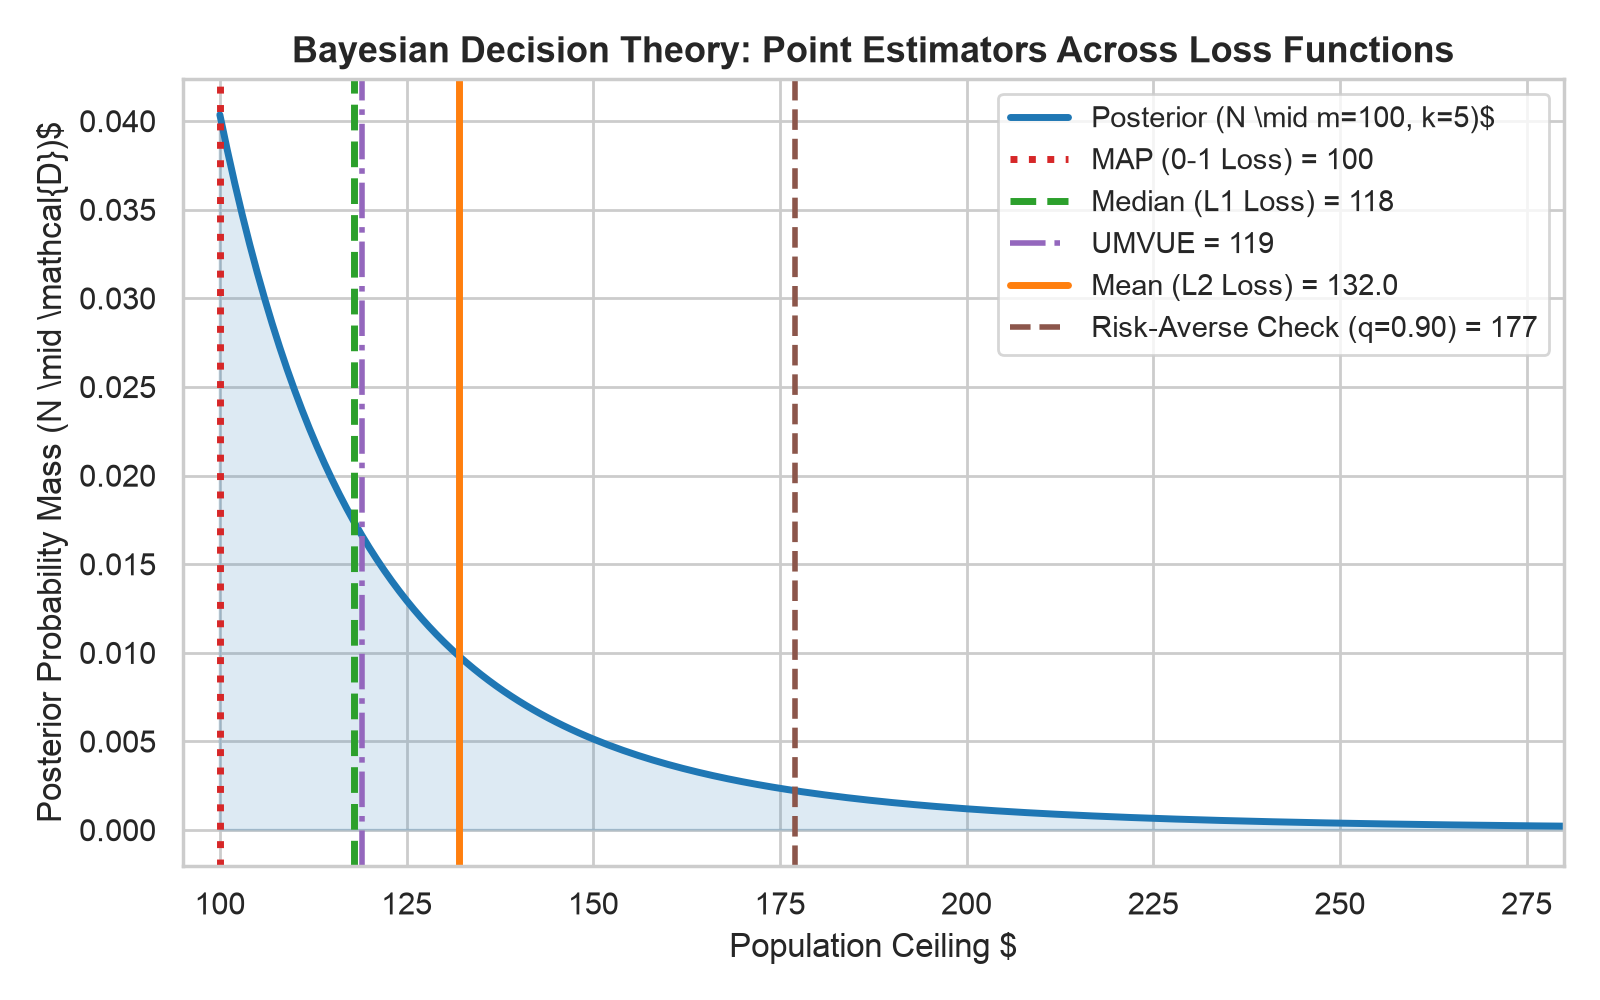
\includegraphics[width=\linewidth,height=0.58\textheight,keepaspectratio]{figures/expert_loss_functions.png}
    \end{column}
    
    \begin{column}{0.50\textwidth}
      {\small \textbf{\color{headernavy} Point Estimates Across Objectives ($m=100, k=5$)}}\\[0.06cm]
      {\scriptsize
      \begin{center}
        \resizebox{\linewidth}{!}{
        \begin{tabular}{llcl}
          \toprule
          \textbf{Objective / Loss} & \textbf{Estimator} & \textbf{Estimate} & \textbf{Strategic Meaning} \\
          \midrule
          0--1 Loss             & MAP / Mode         & \textbf{100} & Extreme lower bound; severe undercount \\
          $L_1$ Absolute Loss   & Posterior Median   & \textbf{118} & Minimizes expected absolute error \\
          $L_2$ Squared Loss    & Posterior Mean     & \textbf{132} & Quadratic balance; tail-inflated \\
          Check Loss ($q=0.90$) & 90th Percentile    & \textbf{175} & $+75\%$ defensive safety buffer \\
          \bottomrule
        \end{tabular}}
      \end{center}
      \vspace{0.08cm}
      \begin{itemize}
        \setlength{\itemsep}{0.08cm}
        \item Under the same observed data ($m=100, k=5$), optimal estimates span from 100 to 175.
        \item Posterior expected loss is minimized at a different point for each loss function.
      \end{itemize}}
    \end{column}
  \end{columns}
  
  \vspace{0.18cm}
  \begin{center}
    {\footnotesize \textbf{\color{headernavy} Key Finding: } \textit{The same observed data can produce vastly different optimal estimates depending on how we value overestimation and underestimation.}}
  \end{center}
\end{frame}

% =========================================================
% Slide 12: Physical Boundary Admissibility: Wald vs Bayesian Intervals
% =========================================================
\begin{frame}[c]
  \begin{center}
    {\large \textbf{\color{headernavy} Physical Boundary Admissibility: Wald vs.\ Bayesian Intervals}}\\[0.10cm]
    {\scriptsize \color{subgray} The physical constraint $N \ge m$ must be respected by any valid uncertainty interval.}
  \end{center}
  \vspace{0.35cm}
  
  \begin{columns}[c,onlytextwidth]
    \begin{column}{0.50\textwidth}
      \centering
      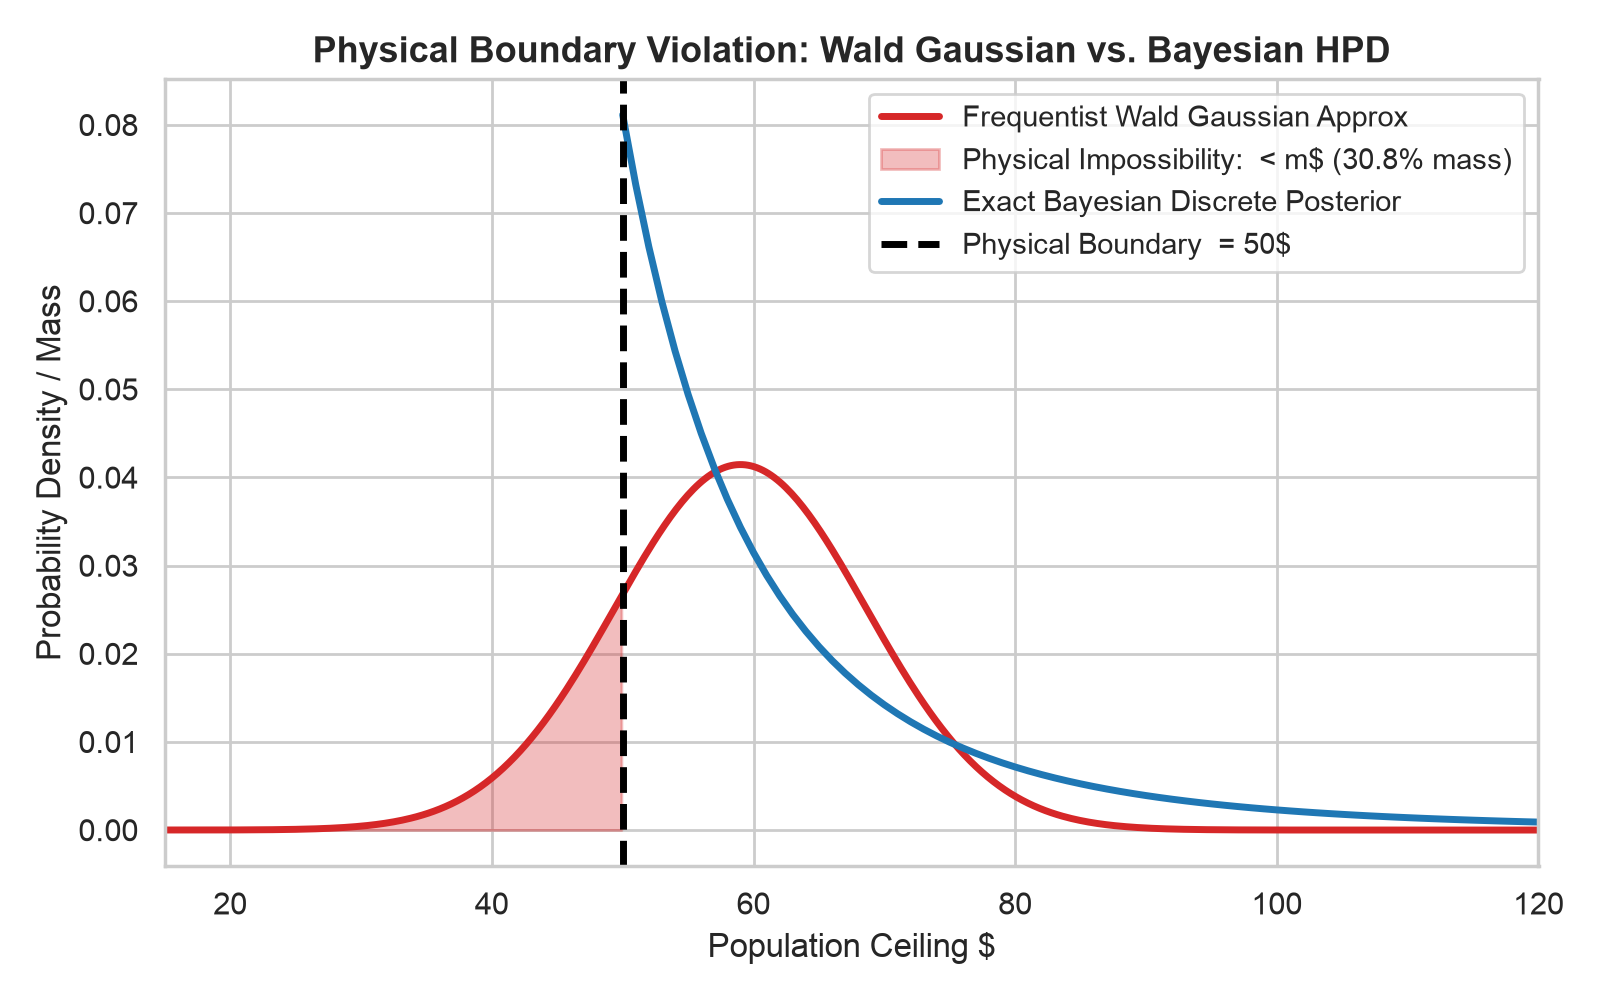
\includegraphics[width=\linewidth,height=0.58\textheight,keepaspectratio]{figures/expert_boundary_wald_vs_bayes.png}
    \end{column}
    
    \begin{column}{0.48\textwidth}
      {\small \textbf{\color{accentred} Frequentist Wald Boundary Collapse}}\\[0.03cm]
      {\scriptsize Wald interval $\widehat{N} \pm 1.96 \cdot \mathrm{SE}$ yields $[40.1, 77.9]$ for $m=50, k=5$. It places \textbf{17.5\% impossible mass} on $N < m=50$. Asymptotic Gaussianity fails completely near the support boundary.}\\[0.12cm]
      
      {\small \textbf{\color{accentgreen} Approximate Frequentist Pivotal CI}}\\[0.03cm]
      {\scriptsize Large-$N$ pivotal interval $[m, m \cdot \alpha^{-1/k}] = [50.0, 91.0]$ respects the physical boundary by construction.}\\[0.12cm]
      
      {\small \textbf{\color{accentblue} Bayesian Credible Coherence}}\\[0.03cm]
      {\scriptsize Reciprocal-prior 95\% credible interval strictly enforces physical admissibility ($P(N < m \mid D) = 0$) and approximately matches the pivotal bound $[50.0, 91.0]$.}
    \end{column}
  \end{columns}
  
  \vspace{0.18cm}
  \begin{center}
    {\footnotesize \textbf{\color{headernavy} Key Finding: } \textit{The reciprocal-prior posterior respects the physical lower bound and produces credible intervals that approximately agree with the large-$N$ frequentist pivotal interval.}}
  \end{center}
\end{frame}

% =========================================================
% Slide 13: Sensitivity to Non-Uniform Sampling: Deployment Tilt
% =========================================================
\begin{frame}[c]
  \begin{center}
    {\large \textbf{\color{headernavy} Sensitivity to Non-Uniform Sampling: When the Maximum Misleads}}\\[0.10cm]
    {\scriptsize \color{subgray} Evaluating estimator robustness when capture probability varies with serial age: $w(s) \propto s^\gamma$.}
  \end{center}
  \vspace{0.35cm}
  
  \begin{columns}[c,onlytextwidth]
    \begin{column}{0.50\textwidth}
      \centering
      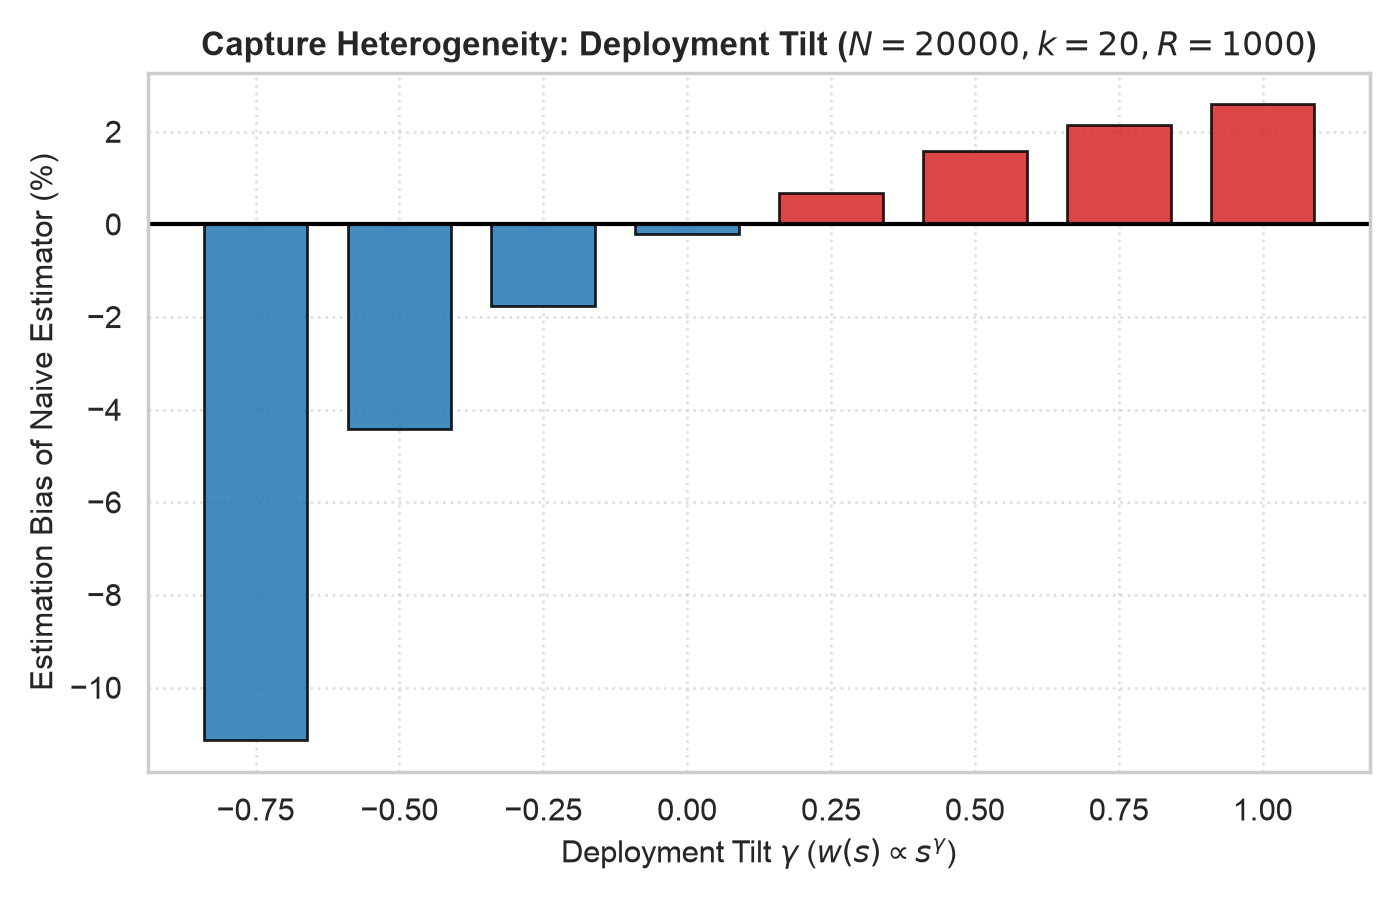
\includegraphics[width=\linewidth,height=0.58\textheight,keepaspectratio]{figures/expert_deployment_tilt.png}
    \end{column}
    
    \begin{column}{0.48\textwidth}
      {\small \textbf{\color{headernavy} Weighted Capture Mechanics}}\\[0.04cm]
      {\scriptsize
      \begin{itemize}
        \setlength{\itemsep}{0.06cm}
        \item $\gamma > 0$ (newer tanks prioritized): pushes $m \to N$, inducing $+1.6\%$ bias at $\gamma = +0.5$.
        \item $\gamma < 0$ (survivorship / depot attrition): induces $-4.4\%$ bias at $\gamma = -0.5$ and $-11.1\%$ bias at $\gamma = -0.75$.
      \end{itemize}}
      \vspace{0.10cm}
      
      {\small \textbf{\color{accentred} Sufficiency Structure Breakdown}}\\[0.04cm]
      {\scriptsize
      \begin{itemize}
        \setlength{\itemsep}{0.06cm}
        \item \textbf{Known $\gamma$:} $m$ remains sufficient for $N$ via tilted factor $g_N(m;\gamma)$.
        \item \textbf{Unknown $\gamma$:} $m$ alone ceases to be sufficient; joint minimal sufficient statistic is $(m, \sum_{i=1}^k \log s_i)$.
      \end{itemize}}
    \end{column}
  \end{columns}
  
  \vspace{0.18cm}
  \begin{center}
    {\footnotesize \textbf{\color{headernavy} Methodological Warning: } \textit{Applying standard estimators when sampling is tilted introduces systematic bias; joint inference over $(N, \gamma)$ is required.}}
  \end{center}
\end{frame}

% =========================================================
% Slide 14: Section 02 Divider (Deep Navy)
% =========================================================
{
\setbeamercolor{background canvas}{bg=navybg}
\begin{frame}[c,plain]
  \centering
  {\scriptsize \textbf{\color{accentcyan} SECTION 02}}\\[0.25cm]
  {\LARGE \textbf{\color{white} Controlled Monte Carlo Simulation Study}}\\[0.35cm]
  {\small \color{white!70} Evaluating bias, RMSE contraction, interval calibration, and prior sensitivity across $R=4,000$ trials ($N=20,000$)}
\end{frame}
}

% =========================================================
% Slide 15: Estimator Bias: Finite-Sample Shrinkage vs Unbiasedness
% =========================================================
\begin{frame}[c]
  \begin{center}
    {\large \textbf{\color{headernavy} Estimator Bias: Finite-Sample Shrinkage vs.\ Unbiasedness}}\\[0.10cm]
    {\scriptsize \color{subgray} Evaluating mean bias convergence across $R = 4,000$ Monte Carlo replications on $N_{\mathrm{true}} = 20,000$.}
  \end{center}
  \vspace{0.35cm}
  
  \begin{columns}[c,onlytextwidth]
    \begin{column}{0.52\textwidth}
      \centering
      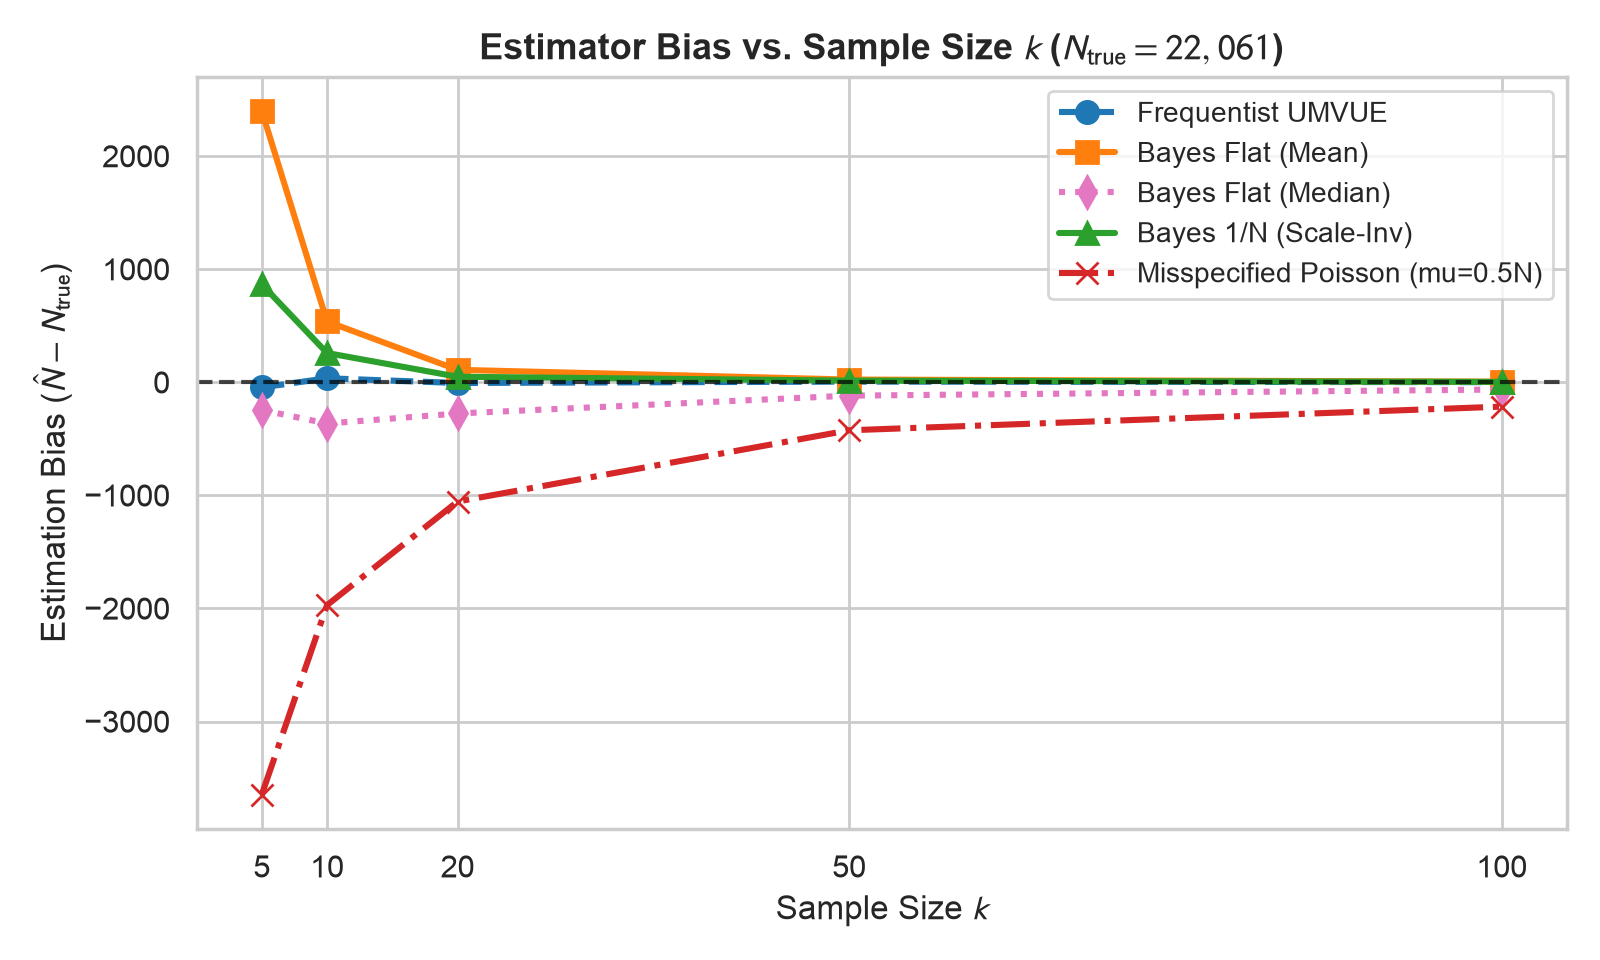
\includegraphics[width=\linewidth,height=0.58\textheight,keepaspectratio]{figures/benchmark_bias.png}
    \end{column}
    
    \begin{column}{0.46\textwidth}
      {\small \textbf{\color{accentgreen} Frequentist UMVUE Unbiasedness}}\\[0.03cm]
      {\scriptsize $\widehat{N} = m(1 + 1/k) - 1$ exhibits near-zero bias across all $k$ ($-48.0 \pm 54.6$ at $k=5$, $+5.2 \pm 6.0$ at $k=50$). Unbiased over hypothetical repeated samples.}\\[0.12cm]
      
      {\small \textbf{\color{accentblue} Bayes Reciprocal Prior}}\\[0.03cm]
      {\scriptsize Posterior Mean has modest bias ($+767.0 \pm 56.8$ at $k=5$), rapidly decaying to $+13.2$ at $k=50$. Posterior Median exhibits negative shrinkage ($-901.5$ at $k=5$).}\\[0.12cm]
      
      {\small \textbf{\color{accentred} Flat Prior Tail Inflation}}\\[0.03cm]
      {\scriptsize Skewed Pareto tail inflates flat posterior mean by $+2,168.6 \pm 60.7$ at $k=5$.}
    \end{column}
  \end{columns}
  
  \vspace{0.18cm}
  \begin{center}
    {\footnotesize \textbf{\color{headernavy} Core Distinction: } \textit{Unbiasedness is a repeated-sampling frequentist property; Bayesian posterior summaries are chosen using the posterior distribution and a decision objective.}}
  \end{center}
\end{frame}

% =========================================================
% Slide 16: Faster-Than-Standard-CLT Error Contraction: RMSE & Variance
% =========================================================
\begin{frame}[c]
  \begin{center}
    {\large \textbf{\color{headernavy} Faster-Than-Standard-CLT Error Contraction: RMSE \& Variance}}\\[0.08cm]
    {\scriptsize \color{subgray} Boundary order-statistic structure accelerates Root Mean Squared Error decay to $\mathcal{O}(k^{-1})$.}
  \end{center}
  \vspace{0.25cm}
  
  \begin{columns}[c,onlytextwidth]
    \begin{column}{0.52\textwidth}
      \centering
      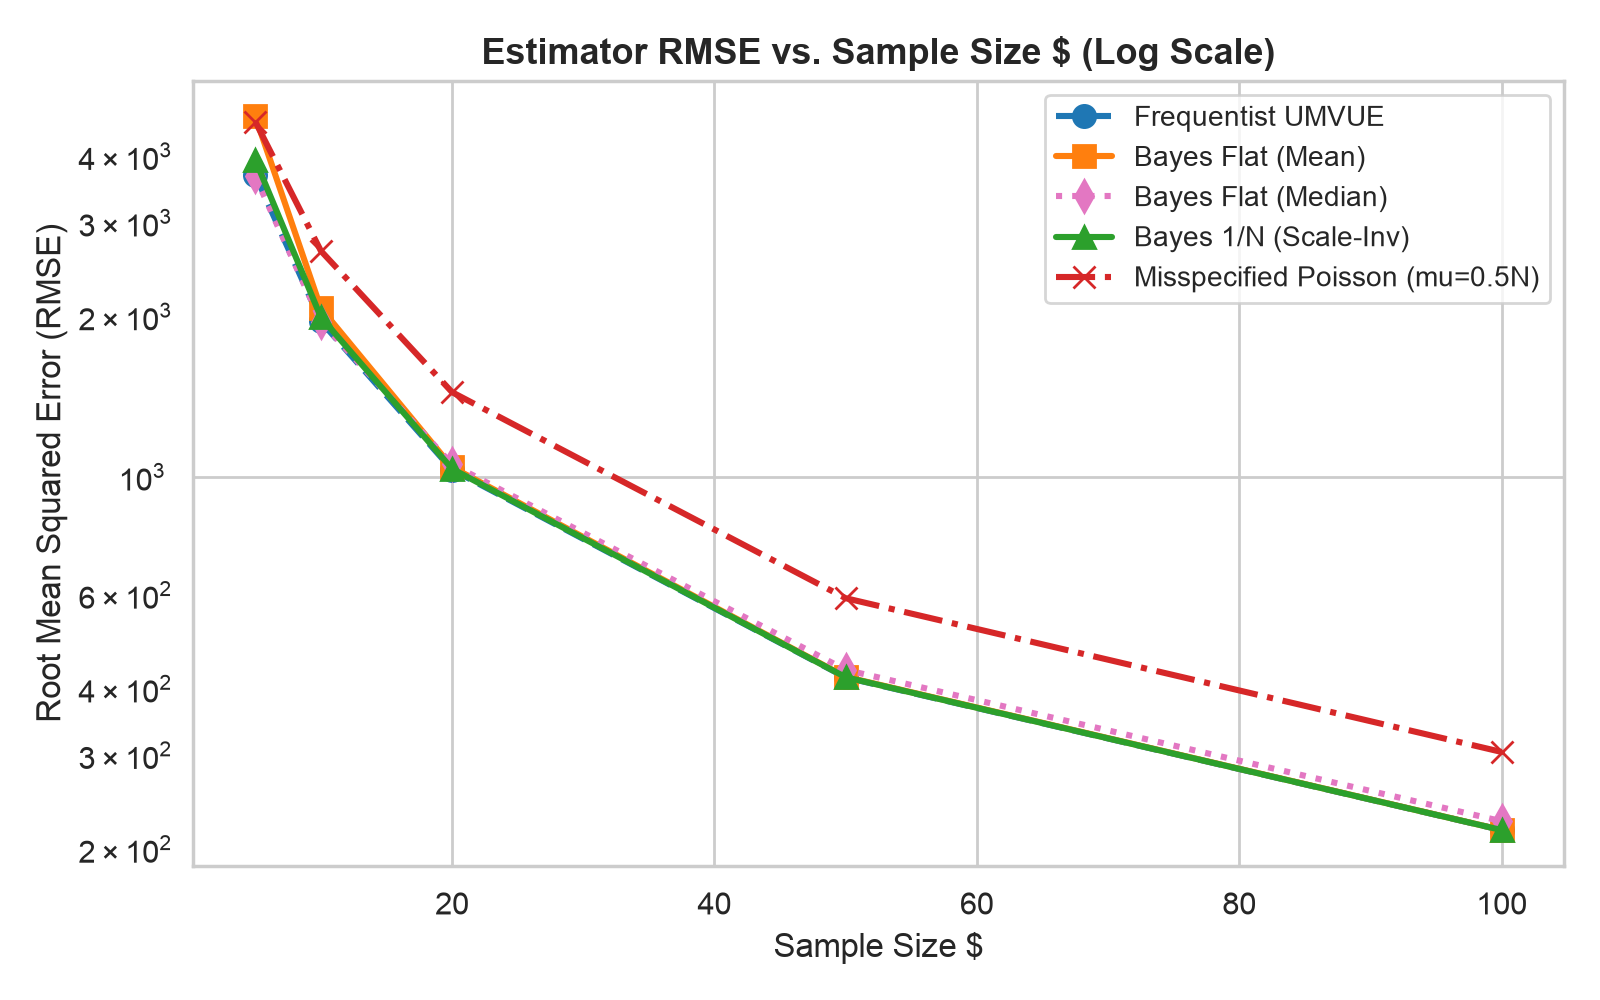
\includegraphics[width=\linewidth,height=0.55\textheight,keepaspectratio]{figures/benchmark_rmse.png}
    \end{column}
    
    \begin{column}{0.46\textwidth}
      {\small \textbf{\color{accentgreen} Theoretical Error Rate}}\\[0.02cm]
      {\scriptsize Because $N$ bounds the support, the UMVUE variance satisfies:
      \begin{equation*}
        \operatorname{Var}(\widehat{N}) = \frac{(N-k)(N+1)}{k(k+2)} = \mathcal{O}(k^{-2})
      \end{equation*}
      giving accelerated rate $\operatorname{RMSE} = \mathcal{O}(k^{-1})$, far outperforming standard CLT rate $\mathcal{O}(k^{-1/2})$.}\\[0.08cm]
      
      {\small \textbf{\color{accentblue} Empirical Concordance}}\\[0.02cm]
      {\scriptsize A $10\times$ increase in $k$ ($5 \to 50$) yields a $\mathbf{9.0\times}$ error reduction ($3,455.2 \to 382.5$), closely matching theoretical $8.6\times$ factor and asymptotic $10\times$ scaling.}\\[0.08cm]
      
      {\small \textbf{\color{headernavy} Estimator Convergence}}\\[0.02cm]
      {\scriptsize For $k \ge 50$, all point estimators achieve identical precision ($\approx 383$).}
    \end{column}
  \end{columns}
  
  \vspace{0.14cm}
  \begin{center}
    {\footnotesize \textbf{\color{headernavy} Contraction Rule: } \textit{The order-statistic boundary structure drives an accelerated $\mathcal{O}(k^{-1})$ RMSE decay, reducing error by nearly an order of magnitude as sample size increases tenfold.}}
  \end{center}
\end{frame}

% =========================================================
% Slide 17: Prior Sensitivity: Calibration and the Informative Trap
% =========================================================
\begin{frame}[c]
  \begin{center}
    {\large \textbf{\color{headernavy} Prior Sensitivity: Calibration and the Informative Prior Trap}}\\[0.10cm]
    {\scriptsize \color{subgray} Evaluating interval reliability and the catastrophic consequences of dogmatic prior misspecification.}
  \end{center}
  \vspace{0.35cm}
  
  \begin{columns}[c,onlytextwidth]
    \begin{column}{0.52\textwidth}
      \centering
      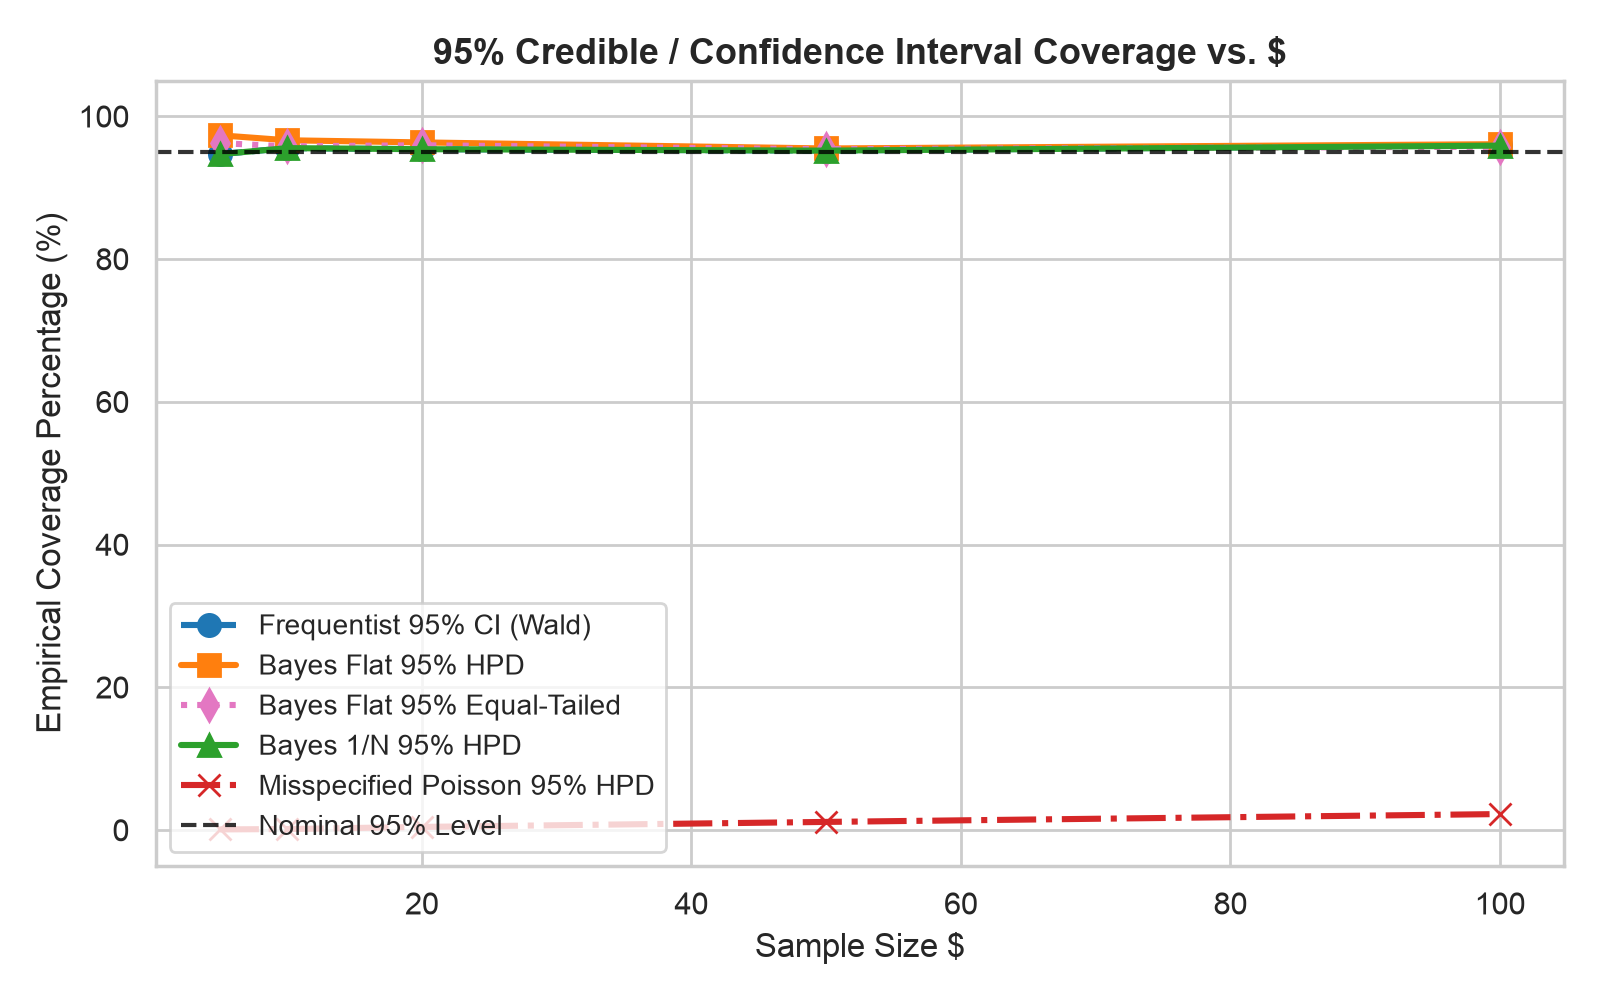
\includegraphics[width=\linewidth,height=0.58\textheight,keepaspectratio]{figures/benchmark_coverage.png}
    \end{column}
    
    \begin{column}{0.46\textwidth}
      {\small \textbf{\color{accentgreen} Reciprocal Prior Calibration}}\\[0.03cm]
      {\scriptsize Empirical coverage closely tracks nominal 95\%: \textbf{94.4\% $\pm$ 0.36\%} at $k=5$ and \textbf{95.6\% $\pm$ 0.32\%} at $k=50$.}\\[0.12cm]
      
      {\small \textbf{\color{accentred} Informative Boundary Trapping}}\\[0.03cm]
      {\scriptsize A dogmatically narrow misspecified Poisson($\mu=10k$) prior traps posterior against the boundary $[m, m+5]$, collapsing coverage to \textbf{0.3\%}.}\\[0.12cm]
      
      {\small \textbf{\color{accentblue} Hierarchical Hyperprior Resolution}}\\[0.03cm]
      {\scriptsize Gamma hyperprior over Poisson rate ($\mathrm{CV} \ge 1$) provides adaptive dispersion, restoring coverage to \textbf{94.6\%--95.0\%} even under 50\% prior mean error.}
    \end{column}
  \end{columns}
  
  \vspace{0.18cm}
  \begin{center}
    {\footnotesize \textbf{\color{headernavy} Calibration Finding: } \textit{The reciprocal prior produces empirical coverage close to 95\% in our simulation. A misspecified Poisson prior causes severe collapse, while a hierarchical prior restores calibration.}}
  \end{center}
\end{frame}

% =========================================================
% Slide 18: Monte Carlo Benchmark: Empirical Performance Leaderboard
% =========================================================
\begin{frame}[c]
  \begin{center}
    {\large \textbf{\color{headernavy} Monte Carlo Benchmark: Empirical Performance Leaderboard}}\\[0.10cm]
    {\scriptsize \color{subgray} Multi-dimensional evaluation across $R = 4,000$ replications on $N_{\mathrm{true}} = 20,000$ (Seed 42).}
  \end{center}
  \vspace{0.30cm}
  
  \begin{center}
    \resizebox{0.92\linewidth}{!}{
    \begin{tabular}{llccccc}
      \toprule
      \textbf{Framework} & \textbf{Estimator} & \textbf{$k$} & \textbf{Mean Bias $\pm$ SE} & \textbf{RMSE (Emp / Th)} & \textbf{95\% Cov $\pm$ SE} & \textbf{Mean Width} \\
      \midrule
      UMVUE (Frequentist)      & $\widehat{N} = m(1 + 1/k) - 1$ & 5  & $-48.0 \pm 54.6$  & 3,455.2 / 3,380.3 & 90.0\% $\pm$ 0.47\% (Wald) & 13,219 \\
      Approximate Pivotal CI   & Large-$N$ Pivotal Bound    & 5  & ---               & ---               & \textbf{94.4\%} $\pm$ 0.36\% & 13,644 \\
      Bayes Flat Prior         & Posterior Mean             & 5  & $+2,168.6 \pm 60.7$& 4,409.0 / 4,363.9 & \textbf{97.4\%} $\pm$ 0.25\% & 18,535 \\
      Bayes Flat Prior         & Posterior Median           & 5  & $-226.5 \pm 54.1$ & 3,431.3 / ---     & \textbf{97.4\%} $\pm$ 0.25\% & 18,535 \\
      Bayes Reciprocal ($1/n$) & Posterior Mean             & 5  & $+767.0 \pm 56.8$ & 3,671.1 / 3,618.6 & \textbf{94.4\%} $\pm$ 0.36\% & 13,622 \\
      Bayes Reciprocal ($1/n$) & Posterior Median           & 5  & $-901.5 \pm 52.3$ & \textbf{3,427.5} / --- & \textbf{94.4\%} $\pm$ 0.36\% & 13,622 \\
      \midrule
      UMVUE (Frequentist)      & $\widehat{N} = m(1 + 1/k) - 1$ & 50 & $+5.2 \pm 6.0$    & 382.5 / 391.8     & 95.1\% $\pm$ 0.34\% (Wald) & 1,536 \\
      Approximate Pivotal CI   & Large-$N$ Pivotal Bound    & 50 & ---               & ---               & \textbf{95.6\%} $\pm$ 0.32\% & 1,211 \\
      Bayes Reciprocal ($1/n$) & Posterior Mean             & 50 & $+13.2 \pm 6.0$   & 382.8 / 392.0     & \textbf{95.6\%} $\pm$ 0.32\% & 1,209 \\
      Bayes Flat Prior         & Posterior Mean             & 50 & $+21.6 \pm 6.1$   & 383.4 / 392.4     & \textbf{95.9\%} $\pm$ 0.31\% & 1,237 \\
      \bottomrule
    \end{tabular}}
  \end{center}
  \vspace{0.18cm}
  
  \begin{columns}[t,onlytextwidth]
    \begin{column}{0.31\textwidth}
      {\small \textbf{\color{headernavy} 1. Point Accuracy}}\\[0.02cm]
      {\scriptsize UMVUE is exactly mean-unbiased; Bayes reciprocal median achieves lowest small-sample RMSE ($3,427.5$).}
    \end{column}
    
    \begin{column}{0.31\textwidth}
      {\small \textbf{\color{headernavy} 2. Interval Reliability}}\\[0.02cm]
      {\scriptsize Reciprocal credible interval achieves $94.4\%$ coverage; Wald interval suffers from boundary distortion ($90.0\%$).}
    \end{column}
    
    \begin{column}{0.31\textwidth}
      {\small \textbf{\color{headernavy} 3. Interval Precision}}\\[0.02cm]
      {\scriptsize Reciprocal intervals are substantially sharper ($13,622$) than flat prior intervals ($18,535$).}
    \end{column}
  \end{columns}
  
  \vspace{0.15cm}
  \begin{center}
    {\footnotesize \textbf{\color{headernavy} Synthesis: } \textit{The reciprocal prior provides a useful balance between estimation accuracy, empirical calibration, and physical admissibility in the simulated setting.}}
  \end{center}
\end{frame}

% =========================================================
% Slide 19: Section 03 Divider (Deep Navy)
% =========================================================
{
\setbeamercolor{background canvas}{bg=navybg}
\begin{frame}[c,plain]
  \centering
  {\scriptsize \textbf{\color{accentcyan} SECTION 03}}\\[0.25cm]
  {\LARGE \textbf{\color{white} Real-World Empirical Stress-Testing}}\\[0.35cm]
  {\small \color{white!70} Evaluating textbook assumptions against WWII archives and 541,909 commercial transactions}
\end{frame}
}

% =========================================================
% Slide 20: Empirical Datasets: Archives & Enterprise Transactions
% =========================================================
\begin{frame}[c]
  \begin{center}
    {\large \textbf{\color{headernavy} Empirical Stress-Testing: Two Real-World Datasets}}\\[0.10cm]
    {\scriptsize \color{subgray} Examining what happens when textbook assumptions meet physical operational systems.}
  \end{center}
  \vspace{0.35cm}
  
  \begin{columns}[t,onlytextwidth]
    \begin{column}{0.48\textwidth}
      {\small \textbf{\color{accentblue} 1. Archival WWII German Tank Ledgers}}\\[0.08cm]
      {\scriptsize
      \begin{itemize}
        \setlength{\itemsep}{0.10cm}
        \item \textbf{Data Source:} Waffenamt ordnance ledgers and Speer Ministry production books.
        \item \textbf{Identifiers Analyzed:} Chassis serial blocks and sequential ZF gearbox stampings.
        \item \textbf{Operational Reality:} Pre-allocated factory blocks; chassis diverted to assault guns (StuG III/IV).
      \end{itemize}}
    \end{column}
    
    \begin{column}{0.48\textwidth}
      {\small \textbf{\color{accentred} 2. Commercial Invoice Ledger (Online Retail)}}\\[0.08cm]
      {\scriptsize
      \begin{itemize}
        \setlength{\itemsep}{0.10cm}
        \item \textbf{Data Source:} 541,909 transaction line items across 4,372 customer accounts.
        \item \textbf{Serials Analyzed:} \textbf{22,061 distinct sequential sales invoices}.
        \item \textbf{Sequence Address Span:} $[536365, 581587] \implies \mathbf{45,223}$ slots.
        \item \textbf{Integer Voids:} $23,162$ unrecorded slots (\textbf{51.2\% void rate}).
      \end{itemize}}
    \end{column}
  \end{columns}
  
  \vspace{0.22cm}
  \begin{center}
    \setlength{\fboxrule}{1pt}
    \fcolorbox{cardborder}{cardbg}{
      \parbox{0.94\textwidth}{\centering
        \scriptsize \textbf{\color{accentred} Crucial Methodological Clarification: }
        These datasets are used to examine the \textbf{limitations of sequential-number inference in operational settings}, NOT to claim that both datasets satisfy the German Tank sampling model.
      }
    }
  \end{center}
  
  \vspace{0.12cm}
  \begin{center}
    {\footnotesize \textbf{\color{headernavy} Distinction: } \textit{541,909 represents raw transaction line items; 22,061 represents distinct sales invoice serial numbers.}}
  \end{center}
\end{frame}

% =========================================================
% Slide 21: Finding 1: Chronological Streaming vs Uniform Sampling
% =========================================================
\begin{frame}[c]
  \begin{center}
    {\large \textbf{\color{headernavy} Finding 1: Chronological Generation vs.\ Uniform Sampling}}\\[0.10cm]
    {\scriptsize \color{subgray} Real-world serials are generated dynamically over time, not drawn as static random samples.}
  \end{center}
  \vspace{0.38cm}
  
  \begin{columns}[t,onlytextwidth]
    \begin{column}{0.48\textwidth}
      {\small \textbf{\color{headernavy} What Was Measured \& Calculated}}\\[0.08cm]
      {\scriptsize
      \begin{itemize}
        \setlength{\itemsep}{0.10cm}
        \item \textbf{Measured:} Arrival timestamps and sequential numeric identifiers across all recorded transactions.
        \item \textbf{Calculated:} Weekly arrival volume $\Delta s / \Delta t$ and cumulative serial growth trajectories.
        \item \textbf{Observed Stream Dynamics:} Weekly volume accelerates from $\approx \mathbf{370}$ invoices/week in Q1 to $>\mathbf{790}$ invoices/week in Q4, peaking at $\mathbf{894}$ invoices/week in mid-November.
      \end{itemize}}
    \end{column}
    
    \begin{column}{0.48\textwidth}
      {\small \textbf{\color{accentred} Research Question Impact \& Statistical Conclusions}}\\[0.08cm]
      {\scriptsize
      \begin{itemize}
        \setlength{\itemsep}{0.10cm}
        \item \textbf{Textbook Assumption:} Assumes a \textit{static population} from which observations are sampled randomly.
        \item \textbf{Operational Reality:} Invoices form an open, chronological transaction stream with non-stationary volume.
        \item \textbf{Exchangeability Violation:} Chronological ordering induces strong temporal autocorrelation. Successive observations are not exchangeable in the way the textbook model assumes.
      \end{itemize}}
    \end{column}
  \end{columns}
  
  \vspace{0.30cm}
  \begin{center}
    {\footnotesize \textbf{\color{headernavy} Statistical Conclusion: } \textit{A static population-ceiling model cannot automatically be applied to a dynamic transaction stream.}}
  \end{center}
\end{frame}

% =========================================================
% Slide 22: Finding 2: Integer Voids & ERP Architecture
% =========================================================
\begin{frame}[c]
  \begin{center}
    {\large \textbf{\color{headernavy} Finding 2: Integer Voids \& System Architecture}}\\[0.10cm]
    {\scriptsize \color{subgray} Operational workflows generate massive integer voids (51.2\% unrecorded rate).}
  \end{center}
  \vspace{0.35cm}
  
  \begin{columns}[t,onlytextwidth]
    \begin{column}{0.48\textwidth}
      {\small \textbf{\color{headernavy} Measured Sequence Breakdown}}\\[0.08cm]
      {\scriptsize
      \begin{itemize}
        \setlength{\itemsep}{0.08cm}
        \item \textbf{Total Integer Address Slots:} $\mathbf{45,223}$ ($s_{\max} - s_{\min} + 1 = 581,587 - 536,365 + 1$).
        \item \textbf{Recorded Sales Invoices:} $\mathbf{22,061}$ ($48.78\%$ recorded).
        \item \textbf{Unrecorded Slots (Voids):} $\mathbf{23,162}$ ($\mathbf{51.22\%}$ void rate).
        \item \textbf{Gap Distribution:} Median gap $\Delta s = 1.0$, mean $2.05$, max $76$.
      \end{itemize}}
    \end{column}
    
    \begin{column}{0.48\textwidth}
      {\small \textbf{\color{accentblue} Verified Facts vs.\ Operational Hypotheses}}\\[0.08cm]
      {\scriptsize
      \begin{itemize}
        \setlength{\itemsep}{0.08cm}
        \item \textbf{Verified Cancellations (3,836):} Exactly 3,836 C-prefixed invoice numbers exist in the raw dataset, directly explaining \textbf{16.56\% of voids}.
        \item \textbf{Operational Hypotheses (19,326):} Without internal server logs, the remaining 83.44\% voids plausibly reflect uncommitted checkout sessions, gateway dropouts, or distributed sequence caching.
        \item \textbf{Wartime Parallel:} Waffenamt pre-allocated chassis blocks; assembly diversions created sequence gaps.
      \end{itemize}}
    \end{column}
  \end{columns}
  
  \vspace{0.28cm}
  \begin{center}
    {\footnotesize \textbf{\color{headernavy} Crucial Distinction: } \textit{The 3,836 cancellations are verified in data; the remaining 19,326 voids are plausible operational hypotheses, not verified findings.}}
  \end{center}
\end{frame}

% =========================================================
% Slide 23: Finding 3: Goodness-of-Fit & The Uniformity Fallacy
% =========================================================
\begin{frame}[c]
  \begin{center}
    {\large \textbf{\color{headernavy} Finding 3: Goodness-of-Fit \& The Uniformity Fallacy}}\\[0.10cm]
    {\scriptsize \color{subgray} Uniform dispersion across an address span is not exchangeability.}
  \end{center}
  \vspace{0.32cm}
  
  \begin{columns}[t,onlytextwidth]
    \begin{column}{0.48\textwidth}
      {\small \textbf{\color{headernavy} What Was Measured \& Calculated}}\\[0.06cm]
      {\scriptsize
      \begin{itemize}
        \setlength{\itemsep}{0.08cm}
        \item Normalized span positions $u_i = (s_i - s_{\min}) / (s_{\max} - s_{\min})$ evaluated against uniform CDF $F(u) = u$.
        \item \textbf{Maximum Absolute Discrepancy:} $D = \sup_u |F_n(u) - u| = 0.012$ ($n = 22,061$).
        \item \textbf{Invalidity of Standard KS Table:} Estimating endpoints from data pins $u_{(1)} = 0$ and $u_{(n)} = 1$. Textbook KS distributions do not apply; formal testing requires parametric bootstrap.
      \end{itemize}}
    \end{column}
    
    \begin{column}{0.48\textwidth}
      {\small \textbf{\color{accentred} What the ECDF Tells Us vs.\ What It Does Not}}\\[0.06cm]
      {\scriptsize
      \begin{center}
        \resizebox{\linewidth}{!}{
        \begin{tabular}{ll}
          \toprule
          \textbf{What the ECDF Tells Us} & \textbf{What It Does NOT Tell Us} \\
          \midrule
          Even distribution across span   & Whether observations are exchangeable \\
          Absence of massive block gaps   & Whether sampling mechanism is uniform \\
          Descriptive numerical regularity& Validity of the German Tank model \\
          \bottomrule
        \end{tabular}}
      \end{center}
      \begin{itemize}
        \setlength{\itemsep}{0.06cm}
        \item A linear ECDF merely shows even allocation across the year.
        \item Successive observations are strongly autocorrelated in time.
      \end{itemize}}
    \end{column}
  \end{columns}
  
  \vspace{0.22cm}
  \begin{center}
    {\footnotesize \textbf{\color{headernavy} Methodological Rule: } \textit{Never interpret a non-significant goodness-of-fit test as proof of exchangeable uniform sampling.}}
  \end{center}
\end{frame}

% =========================================================
% Slide 24: Finding 4: Estimand Disambiguation & Thinning Models
% =========================================================
\begin{frame}[c]
  \begin{center}
    {\large \textbf{\color{headernavy} Finding 4: Estimand Disambiguation \& Thinning Models}}\\[0.10cm]
    {\scriptsize \color{subgray} What exactly are we trying to count? Sequence capacity vs.\ realized transaction volume.}
  \end{center}
  \vspace{0.35cm}
  
  \begin{columns}[t,onlytextwidth]
    \begin{column}{0.48\textwidth}
      {\small \textbf{\color{accentred} Estimand Disambiguation}}\\[0.06cm]
      {\scriptsize
      \begin{itemize}
        \setlength{\itemsep}{0.08cm}
        \item \textbf{Estimand A ($N_{\mathrm{span}} = \mathbf{45,223}$):} Total allocated address capacity ($s_{\max} - s_{\min} + 1$). Raw estimator without base offset yields $\approx 593k$.
        \item \textbf{Estimand B ($N_{\mathrm{count}} = \mathbf{22,061}$):} Net volume of realized, active completed items. Shifting by $s_{\min}$ gives $\mathbf{+105\%}$ error over active count.
        \item \textbf{Oracle Trap:} Rank re-indexing requires knowing all valid keys in advance (un-deployable in live audits).
      \end{itemize}}
    \end{column}
    
    \begin{column}{0.48\textwidth}
      {\small \textbf{\color{accentgreen} The Bernoulli Thinning Model \& Caveats}}\\[0.06cm]
      {\scriptsize
      \begin{equation*}
        N_{\mathrm{count}} \mid N_{\mathrm{span}}, \rho \sim \mathrm{Binomial}(N_{\mathrm{span}}, \rho)
      \end{equation*}
      \begin{itemize}
        \setlength{\itemsep}{0.08cm}
        \item \textbf{Retrospective Calculation:} Using the complete dataset ($k = 22,061$), $\widehat{\rho}_{\mathrm{retrospective}} = \frac{22,060}{45,222} \approx 0.4878$.
        \item \textbf{Operational Identifiability Caveat:} This calculation uses the complete observed invoice set. In an incomplete field sample ($k \ll N$), the sample spacing ratio estimates sample density, not $\rho$.
        \item Estimating both $N_{\mathrm{span}}$ and $\rho$ from an incomplete sample requires auxiliary data.
      \end{itemize}}
    \end{column}
  \end{columns}
  
  \vspace{0.25cm}
  \begin{center}
    {\footnotesize \textbf{\color{headernavy} Conceptual Takeaway: } \textit{Bernoulli thinning clarifies the estimand distinction conceptually; estimating both capacity and void rate requires auxiliary identifying structure.}}
  \end{center}
\end{frame}

% =========================================================
% Slide 25: Discussion: Connections to Other Areas of Inference
% =========================================================
\begin{frame}[c]
  \begin{center}
    {\large \textbf{\color{headernavy} Connections to Other Areas of Statistical Inference}}\\[0.10cm]
    {\scriptsize \color{subgray} How discrete order-statistic inference connects across domains, and where its boundaries lie.}
  \end{center}
  \vspace{0.35cm}
  
  \begin{columns}[t,onlytextwidth]
    \begin{column}{0.48\textwidth}
      {\small \textbf{\color{accentblue} Conceptual Cross-Domain Connections}}\\[0.08cm]
      {\scriptsize
      \begin{itemize}
        \setlength{\itemsep}{0.08cm}
        \item \textbf{Dynamic Production:} Monotonic state-space models ($N_t \ge N_{t-1}$) enforce output non-negativity across periods.
        \item \textbf{Software Reliability:} Jelinski--Moranda defect exhaustion models mirror serial discovery for software release readiness.
        \item \textbf{Aviation Safety:} Beta--Bernoulli mixtures detect cloned counterfeit serial numbers in critical parts supply chains.
        \item \textbf{Wildlife Abundance:} Two-stage cascades infer tag loss before estimating population size via mark-recapture.
      \end{itemize}}
    \end{column}
    
    \begin{column}{0.48\textwidth}
      {\small \textbf{\color{accentred} Methodological Boundaries}}\\[0.08cm]
      {\scriptsize
      \begin{itemize}
        \setlength{\itemsep}{0.08cm}
        \item \textbf{Non-Sequential Keys:} Randomized UUIDv4 or cryptographic hashes completely destroy order-statistic sufficiency.
        \item \textbf{Non-Random Gaps:} Classified blocks or unrecorded overseas entities require informative gap priors.
        \item \textbf{Dynamic Streams:} Fast-changing arrival rates require time-varying Poisson arrival processes.
        \item \textbf{Identifiability Limits:} Incomplete samples cannot simultaneously identify capacity and void rate without auxiliary data.
      \end{itemize}}
    \end{column}
  \end{columns}
  
  \vspace{0.25cm}
  \begin{center}
    {\footnotesize \textbf{\color{headernavy} Synthesis: } \textit{Order-statistic inference generalizes broadly across domains, provided analysts explicitly model data-generating mechanisms and respect identifiability boundaries.}}
  \end{center}
\end{frame}

% =========================================================
% Slide 26: Summary & Key Conclusions (Deep Navy)
% =========================================================
{
\setbeamercolor{background canvas}{bg=navybg}
\begin{frame}[c,plain]
  \centering
  {\scriptsize \textbf{\color{accentcyan} SUMMARY \& CONCLUSIONS}}\\[0.12cm]
  {\Large \textbf{\color{white} Key Takeaways for Bayesian Discrete Inference}}\\[0.40cm]
  
  \begin{columns}[t,onlytextwidth]
    \begin{column}{0.31\textwidth}
      \centering
      {\small \textbf{\color{accentcyan} 1. Objective Foundations}}\\[0.10cm]
      {\scriptsize \color{white!85} The target is the discrete ceiling $N$, with evidence captured by sample maximum $m$. Scale-invariant reciprocal prior $\pi(N) \propto 1/n$ yields proper posteriors ($k \ge 1$), respects physical boundaries ($N \ge m$), and matches the large-$N$ pivotal bound.}
    \end{column}
    
    \begin{column}{0.31\textwidth}
      \centering
      {\small \textbf{\color{accentcyan} 2. Decision Theory \& Rates}}\\[0.10cm]
      {\scriptsize \color{white!85} Point estimation follows loss geometry: median minimizes absolute error; check loss ($q=0.9$) builds defensive buffers. Extreme-value order statistics produce accelerated $\mathcal{O}(k^{-1})$ RMSE contraction ($9\times$ reduction for $10\times$ sample).}
    \end{column}
    
    \begin{column}{0.31\textwidth}
      \centering
      {\small \textbf{\color{accentcyan} 3. Real-World Reality}}\\[0.10cm]
      {\scriptsize \color{white!85} Operational data violate textbook assumptions via chronological streaming and integer voids (51.2\%). Bernoulli thinning disambiguates address capacity from realized transaction volume.}
    \end{column}
  \end{columns}
  
  \vspace{0.35cm}
  \begin{center}
    \setlength{\fboxrule}{1pt}
    \fcolorbox{cardborder}{navybg!80!white}{
      \begin{minipage}{0.92\textwidth}
        \centering
        \scriptsize \color{white}
        \textbf{Central Research Answer: } Bayesian inference provides a principled framework for quantifying uncertainty about an unknown discrete population ceiling, selecting estimates under mission-specific decision objectives, and evaluating inferential reliability. Its practical validity in the physical world, however, depends entirely on whether operational data-generation mechanisms satisfy model assumptions.
      \end{minipage}
    }
  \end{center}
  
  \vspace{0.20cm}
  {\scriptsize \color{white!60} Aklanta Borah, Amartya Amritanshu, Rajveer Vora --- Indian Statistical Institute, Kolkata (Nov 2026)}
\end{frame}
}

\end{document}
